This chapter presents the background and related work. In Section~\ref{sec:background}, we introduce the background of this thesis. This includes a brief introduction of the development of artificial intelligence (AI), how AI and robotics are combined, and the research that has been done in recent years in the areas of automation science. Section~\ref{sec:evolutionary_computation} reviews the development of evolutionary computation which is the main technique used in this thesis. This section includes an introduction of biological evolution, \textcolor{red}{principles, strengths and caveats of evolutionary computing} and its applications. Section~\ref{sec:combine_AI_robotics_animal_behavior} introduces how AI/robotics and animal behavior study benefit from each other, which includes how animal behavior can be used as inspiration for AI and robotics and the methods to investigate animal behavior using AI/robotics techniques.  
%As the theme of this thesis is to show how machine intelligence can be used for learning agent behaviors, Section~\ref{sec:animal_behavior_in_nature} presents some examples of animal behaviors observed in nature. Section~\ref{sec:swarm_optimization_swarm_robotics} reviews how animal behavior can be used as inspiration for AI and robotics. Section~\ref{sec:contribution_of_AI/robotics_to_ethology} reviews two methods to study animal behaviors using AI/robotics techniques.  

\section{Background}\label{sec:background}

\subsection{The Development of AI and Robotics}\label{sec:development_of_AI_Robotics}

Intelligence is a natural part of life. Humans and other biological creatures exhibit many intelligent behaviors such as pattern recognition and decision making. However, intelligence is not a property that is limited to biological creatures. It should be equally applicable to computers or machines. The term AI emerged in a conference in 1956 at Dartmouth College, where several pioneers of this filed including Marvin Minsky, John McCarthy, etc., discussed the development of digital computer and the future of AI. The definition of AI is still a disputed topic.  Some researchers argued that AI is to simulate the intelligent behaviors which are observed in humans and other biological creatures using computers or machines. That is, an intelligent machine should be able to exhibit behaviors similar to that of humans when encountering the same problems~\cite{Schildt1985}. Others gave the following definition: ``Artificial Intelligence is the study of mental faculties through the use of computational models''~\cite{Charniak1985}. According to Fogel~\cite{Fogel1995}, an intelligent system should know how to make decision in order to fulfill a goal (e.g., solving a problem). In other words, instead of pre-programming the machine using human's knowledge, the machine should be able to learn and adapt. In~\cite{Minsky_1991}, Minsky even argued, ``Why can't we build, once and for all, machines that grow and improve themselves by learning from experience? Why can't we simply explain what we want, and then let our machines do experiments or read some books or go to school, the sorts of things that people do?'' In 1950, Turing~\cite{Turing_1950} proposed an imitation game which is nowadays known as \textit{Turing test} to discuss a question: ``Can machine think?''. Although whether a machine could pass the \textit{Turing test} or not is beyond the consideration at that time, it was accepted as a notion that a machine could mimic human behavior. Many promising achievements have been made to enable machines to do a variety of intelligent things since then. 

In the 1970s, the emergence of expert system~\cite{Jackson1998}, which mimics a human expert's decision-making capability, significantly promoted the development of AI. These expert systems can solve complicated problems through reasoning mainly based on \textit{if-else} rules. One of the most representative examples is IBM's chess program (Deep Blue). It defeated the champion of the world chess (Gary Kasparov) in 1997~\cite{Newborn1992}, which provides evidence that a computer program can outperform a human expert in term of decision-making ability. An expert system consists of two components: knowledge base and inference engine. Knowledge base contains facts and rules that are known to the system. Inference engine uses the knowledge to make decision and derive some new rules. The rules in expert systems can be absolute or fuzzy. Expert systems have many commercial applications such as medical diagnosis \cite{Buchanan:1984}, prediction \cite{Robert1993} and monitoring \cite{Salvaneschi1996}, etc. Fuzzy logic was first introduced by Zadeh~\cite{Zadeh:IC:1965} to describe element in a range rather than give an absolute value. This is common in our daily life. For example, in stock market an old saying is: ``buy low, sell high''. However, whether the stock value can be considered as low or high depends on the stock curves in a particular situation. Fuzzy systems have many commercial applications in such as air conditioner, digital camera and and hand writing recognition, etc. Another representation of machine intelligence is neural network, which mimics the processing ability of nervous systems of biological creatures (especially human brain). Through a combination of weights and excitation functions (e.g., sigmoid function), neural networks can accomplish many tasks observed in humans, such as pattern recognition and image processing. 

%Over decades, researchers are dedicated to making machine exhibit behaviors using symbolic representations to mimic human behaviors. The rules executed in a machine are usually programmed. However, when we consider the natural evolutionary process, it takes ages for humans to pick up a particular intelligence behavior. It is straightforward to say that through simulating the natural evolutionary process, a machine could exhibit intelligence that may be unpredictable by the programmers~\cite{Fogel1995}. In other words, intelligence can be evolved, and this is the main topic discussed in the rest of this thesis. 
%In 1959, a program was written to play checkers~\cite{Samuel1959}. 

%In the early stage of AI, the program is only run on a computer, and the input is digital. With the development of AI and hardware, researchers start to combine AI with moving machines such as a robot. Different from the digital world in a computer, the environment that a robot operates on is much more complex. The input of the system can be digital, analog or hybrid, which makes the modeling/abstract of the operating environment challenging. 
Robotics is about making the machines that can move in a number of ways in order to accomplish different tasks. While AI and robotics are not essentially connected, they are often used together to make the robots smarter. For example, a robot with AI can move autonomously and makes decision while interacting with the environment it is operating on. Through combining AI and robotics, machines can be made to behave more like humans or animals. Instead of only executing programmed code as in a car assembling line, robots can learn and adapt to the changing environment.

There are two common architectures adapted for the control of a robot: deliberative architecture and subsumption architecture~\cite{Brooks1986}. In deliberative architecture, the robot operates on a top-down fashion and its action mainly depends on planning. A typical cycle is: $sensor \rightarrow plan \rightarrow act$. In the sensor stage, the robot gets the information from the world based on sensors such camera, infrared sensors. After pre-processing, this information would be passed to the central control architecture which integrates all the sensing information and reasons about it. Based on the knowledge the robot has to decide which action to take next to fulfill a goal (e.g., maximize its reward). This architecture has led to many successful applications. The pioneer work is~\textit{Shakey the robot} which is capable of reasoning about its own actions~\cite{Nilsson1984}. In this work, the environment the robot is operating on is simplified and the experimental conditions are well controlled (e.g. uniform color and flat floor). More work has been done since then to enable robots to tackle complex and changing environments. Another architecture adapted widely nowadays is subsumption architecture~\cite{Brooks1986}, in which the robot makes decision based on $sensor \rightarrow act$ without deliberate reasoning or planing. Instead of building a central reasoning system to integrate all the sensory information, the robot could process it in parallel by each layer. This could enhance the robustness of the robotic control system.  Some famous robots using subsumption architecture are Allen, Herbert and Genghis (to list a few). 
%To accomplish a complex task, researchers may need to combine different architectures integrated in a cognitive manner. This lead to a new research area---cognitive robotics. It is argued that intelligence emerges from interaction of different layers of $sensor \rightarrow act$ pairs.
 
\subsection{Introduction of Automation Science}

Since intelligent and automation systems were used by researchers in laboratory automation~\cite{Sasaki_1998} in the early 1980s to analyze huge number of samples a day, such systems are increasingly used in agriculture, chemistry and energy labs, etc. Nowadays, it is the demand that machines could automate the whole process of scientific experiments. The question of whether it is possible to automatically conduct scientific research is very interesting in theory, and it also involves a lot of practical work which needs to be solved. In order to speed up experimental process, researchers should take advantage of machines/robots to help, for example, collect and analyze thousands of data, because these things are very time-consuming and boring if only carried out manually. The ideal situation is to make a machine do the experiments automatically without or with little human intervention. Such kind of machine can do experiments day and night in a constant manner without any tiredness and complain.
          
The field of automation science has been developed to a great extent because of the increasing demands of drug industry and relevant fields of biology and chemistry. High-throughput screening (HTS) system~\cite{Persidis_1998} is one of the early efforts. The HTS system could do many things such as preparation, observation and analysis of assay, greatly enhancing the speed of data collection and analysis process in a short time. Recently, King, et al. have built a Robot Scientist---Adam,  which can automatically generate functional genomics hypotheses about the yeast~\textit{Saccharomyces cerevisiae} and carry out experiments to test and refine the hypotheses based on the approaches from artificial intelligence~\cite{King_2004, King_2009}. This Robot Scientist is able to do plenty of experiments and observations a day. The experiments are initialized and done automatically by machines, which makes it possible to test all aspects of experimental process. Adam could automatically conduct the cycles of scientific experiments: forming hypothesis, initializing the experiments, explaining the results and verifying the hypothesis, and then repeating the cycle. The functional genomics hypotheses are autonomously generated by intelligent software and the experiments are conducted by various technologies based on AI research~\cite{King_2004}. Therefore, Adam is the integration of robotic system, automatic control technology as well as artificial intelligent. 

In system identification area, Gauld et al. have developed a digital automated identification system (DAISY) to identify biological species automatically with high accuracy using advanced image processing technique~\cite{Gauld_2000}. This kind of technology has gone though great improvement in recent years, raising the possibility of automation, or at least semi-automation, in the process of routine taxonomic identification. In~\cite{MacLeod_2010}, MacLeod et al. report that an imaging system that is originally designed for identifying marine zooplankton was used by the US government for monitoring horizon oil spill in the deep water. They argue that taxonomists and researchers in machine learning, pattern recognition as well as artificial intelligence should collaborate with each other in order to better identify and name biological species. 

Drawing on approaches from various research areas especially artificial intelligence, intelligent and automation systems are playing a vital role in scientific research, allowing researchers to conduct experiments more efficiently. It is argued that the revolution of automation science will emerge in a few decades~\cite{King_2009}.

\section{Evolutionary Computation}\label{sec:evolutionary_computation}

Evolutionary computation is a technique which draws inspiration from biological evolution. Evolutionary computation is a population-based search/optimization method, and it typically uses the trial-and-error to guide the search process. It is a stochastic search method and not task-dependent. In Section~\ref{sec:natural_evolution}, we briefly introduce the natural evolution, including evolution and coevolution. In Section~\ref{sec:intro_evolutionary_computation}, we detail the principles of evolutionary algorithms and coevolutionary algorithms. Section~\ref{sec:application_evolutionary_computation} presents three main applications of evolutionary computation and the related work in this thesis.

\subsection{Biological Evolution}\label{sec:natural_evolution}

%\subsubsection{Evolution}

Natural evolution deals with the questions of how creatures evolve to adapt to their changing environment. According to Darwin's Theory of Evolution~\cite{Darwin_1859}, species fight for survival. The species that can fit the environment survive, and others that can not would die. This phenomenon is regarded as~\textit{survival of the fittest} or~\textit{natural selection}. There are heritage (e.g. through sexual reproduction) and random mutation among species's genes. The genes that help the species survive would be preserved and passed on to the next generation, and the genes that are harmful or not useful would be abandoned. %This is called natural selection. 

Natural selection tends to reserve and accumulate small beneficial genetic mutations. Suppose that some members in a species have evolved a functional organism that is very useful (e.g., a wing that can fly). This makes these creatures easier to find food or avoid threat from predators. Their offspring are more likely to inherit such advantageous function and this function would be passed to the next generation. The other members without the advantageous function are more likely to die out. Natural selection helps the species to compete and adapt better in the environment. At the same time, it also accelerates the extinction of the species that can not fit the environment. The dinosaur used to be a dominant species in the ancient world due to the big body and ability of flying. This was a big advantage when the climate is mild. However, once the climate changed and became much hotter, the big body is no longer an advantage as it needs to consume much more energy. This led to the extinction of this species. On the hand hand, the flying creatures with small body such as birds survived from the climate change. 

%\subsubsection{Coevolution}

Coevolution is special form of evolution, which involves in the simultaneous evolution of two or more species. A typical example of natural coevolution is fox and rabbit or parasite and host. In nature, the survival ability between individuals is coupled. That means the survival ability of one particular individual depends not only on its chromosome, but also the interaction with other individuals. The creatures which exist separately in a certain time or space, have various relationships between each other. Although the correlation between different species is complicated, for a specific species, there are three possibilities: beneficial, injured and neutral. Therefore, through permutation and combination, the relationship between two species can be summarized in Table~\ref{tab:relationship_species_coevolution}. It includes 6 concrete relationship: reciprocity, neutral, symbiosis, amensalism, predation and antibiosis.

\begin{table}[!t]          
  \centering                     
  \caption{The relationship between different species}
  \label{tab:relationship_species_coevolution} 
  \renewcommand{\arraystretch}{1.5}
  \begin{tabularx}{400pt}{l|l|l|l}                                                    
    \hline                                                                %\hline: the herizon line
     & \multicolumn{3}{c}{the influence of species A } \\                       % use & to divide the columns         
    \hline
    & +,+ (reciprocity)  & +,0 (symbiosis)   & +,- (predation)   \\
    the influence of species B & 0,+ (symbiosis) & 0,0 (neutral) & 0,- (amensalism)  \\
    & -,+ (predation)    & -,0 (amensalism) & -,-(antibiosis) \\
    \hline
  \end{tabularx}
\end{table}

Where, symbol '+', '-' and '0' represent beneficial, injured and neutral. For example, ``+, -'' indicates A benefits and B gets injured in the relationship.

\subsection{Introduction of Evolutionary Computation}\label{sec:intro_evolutionary_computation}

\subsubsection{Evolutionary Algorithms}

Based on the principle of biological evolution, a bi-inspired algorithm ---  genetic algorithm (GA) was proposed by Halland in 1960s \cite{Halland_1992}. GA simulates the heritage, mating, and mutation of the natural evolution. In GA, the solution for a given problem is represented as chromosome, which contains several genes. Each gene could be a binary number, integer, or floating-point number. Heritage is also called reproduction in GA. Mating corresponds to crossover/mate, in which different individuals exchange genes. Mutation is normally realized by randomly changing a particular gene. For example, some gene in the chromosome may be randomly replaced by another gene. Mutation in GA serves the same function as it is in natural evolution. It creates the diversity and creativity. Unlike natural evolution which does not have a specific goal, GA is driven by a fitness function. The evolutionary process is to optimize (e.g., maximize) the fitness of the individuals in the population. There are other types of evolutionary algorithms that based on the basic idea of natural evolution. Fogel, Owens and Walsh invented \textit{evolutionary programming (EP)}~\cite{Fogel1966}. Rechenberg and Schwefel introduced \textit{evolution strategies (ES)}~\cite{Rechenberg1994}, which are mainly dealing with real-value continuous optimization problem. In the early 1990s, another new evolutionary algorithm called \textit{genetic programming (GP} was presented by Koza~\cite{Koza1992}. Fig.~\ref{fig:evolutionary_algorithm_classification} shows a brief classification of evolutionary algorithms. 

\begin{figure}[htbp]
  \centering
  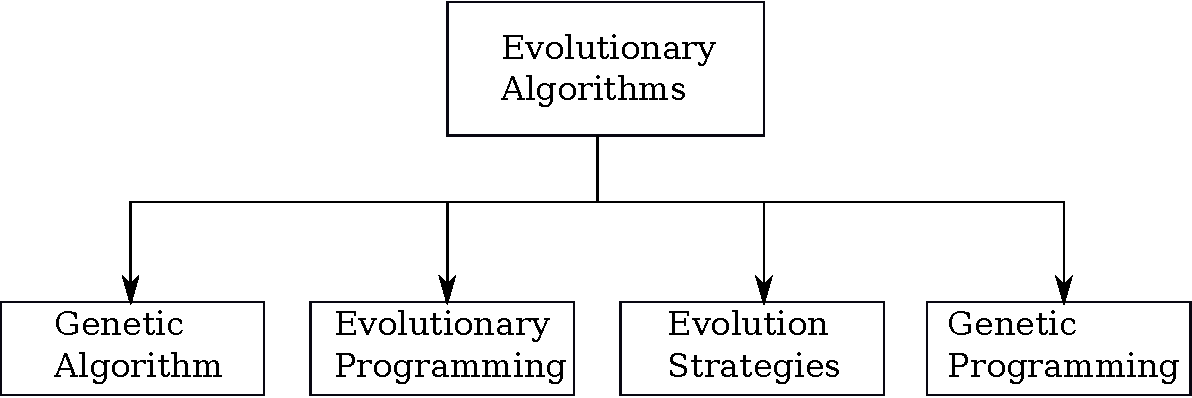
\includegraphics[width=4.2in]{evolutionary_algorithm_classification.pdf}
  \caption{Classification of evolutionary algorithms}
  \label{fig:evolutionary_algorithm_classification}
\end{figure}

The implementation of evolutionary algorithms follow a general flow during the operation process. They can be divided into $5$ steps: initialization, evaluation, mutation, selection and termination. At the beginning, a random population of individuals is initialized. These could be several random strings (chromosomes or individuals), each of which contains several genes (e.g. floating point number). These strings are encoded of the solutions we want to get. Different chromosomes are then evaluated using certain fitness function. Selection happens after the evaluation of each individual, and the ones with higher fitness normally have a higher chance of being selected to be passed to the next generation or have offsprings. The offsprings have the chance of mutation to generate new genes.  Fig.~\ref{fig:evolutionary_algorithms_flow} show a diagram of how the evolutionary algorithms proceed. 

\begin{figure}[htbp]
  \centering
  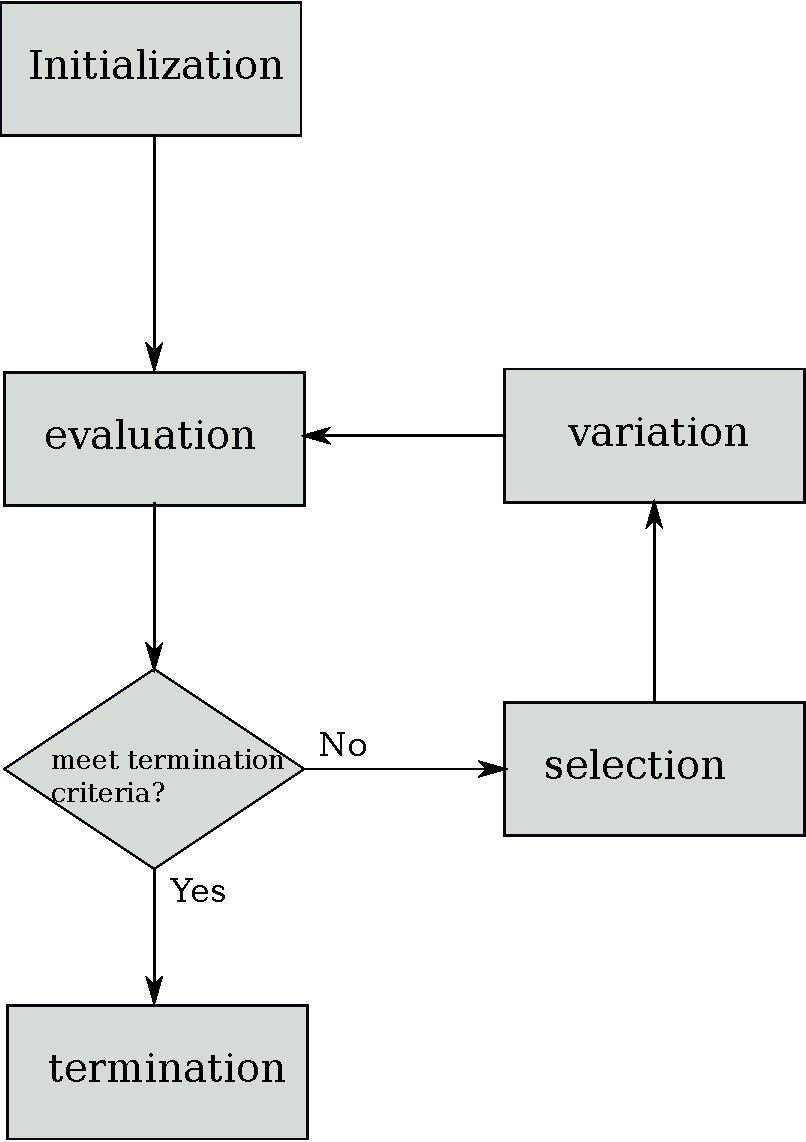
\includegraphics[width=2.0in]{evolutionary_algorithms_flow.pdf}
  \caption{This diagram shows the flow of evolutionary algorithms.}
  \label{fig:evolutionary_algorithms_flow}
\end{figure}
%For example, genetic algorithms have been applied to automatic design of mechatronic systems, complicated trading system, etc. 

\subsubsection{Coevolutionary Algorithms}

\textit{1) Principles of Coevolutionary Algorithms:} In genetic algorithm, the fitness of individuals is only decided by their own chromosomes. That means in different generations, the fitness of individuals who own the identical chromosome is constant. However, this is not true in natural coevolution. The creatures in nature are not independent, and they have different kinds of relationship as shown in Table~\ref{tab:relationship_species_coevolution}. The evolution of individuals among different species as well as evolution within the same species are coupled. Based on the idea of ecological coevolution, the coevolutionary algorithms are widely used in various research areas \cite{Rosin_1997}. Figure \ref{Fig: diagram_coevolution} shows the schematic diagram of coevolutionary algorithms between two different populations. In principle, coevolutionary algorithms can be considered of comprising several sub-algorithms, each of which could be an evolutionary algorithm. These sub-algorithms interact with each other in the fitness calculation process. In other words, the fitness of individuals in one population not only depends on its own chromosome, but also on the performance of other individuals from another population during the coevolutionary process. 

\begin{figure}[htbp]
  \centering
  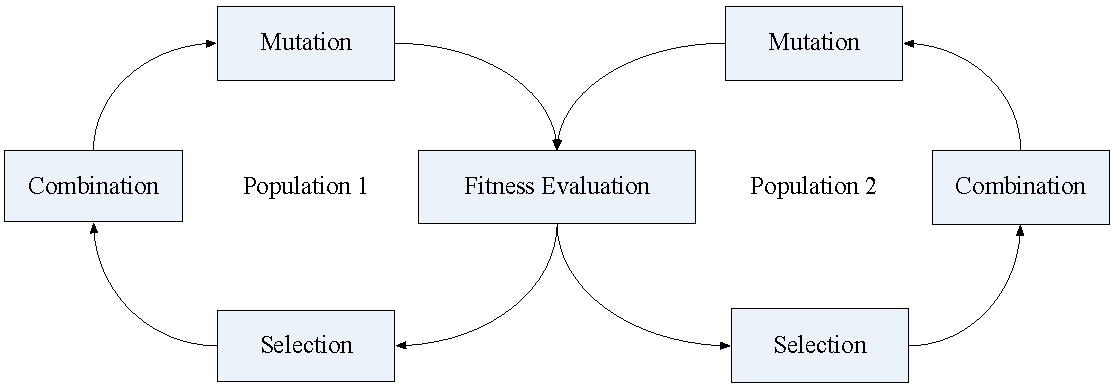
\includegraphics[width=4.2in]{diagram_co_evolution.pdf}
  \caption{Schematic diagram of coevolutionary algorithms between two different populations.}
  \label{Fig: diagram_coevolution}
\end{figure}

The essential difference between evolutionary algorithms and coevolutionary algorithms is the way of fitness evaluation. Standard genetic algorithms evaluate individuals by their chromosomes, which are independent of those in other individuals in the evolutionary system. Coevolutionary algorithms evaluate individuals based on their relative performance compared with other individuals. According to the way of evaluation, the coevolutionary algorithms are generally divided into two categories---competitive coevolutionary algorithm (Comp-CEA) and cooperative coevolutionary algorithm (Coop-CEA). Comp-CEA assesses each individual by its competitive performance with respect to its opponents, while Coop-CEA assesses each individual by its cooperative performance with respect to its co-operators. As discussed by Dawkins and Krebs \cite{Dawkins_1979}, competitive coevolution can produce a phenomena of ``arm races'' by increasing the complex of each population in the coevolution. The evolution of one species may drive another species to evolve new strategies, which makes both of the species evolve a higher level of complex behavior. Generally, Coop-CEA is applied to the situation in which the problem can be divided into several sub-problems. In Coop-CEA, thare are several cooperative species evolving simultaneously, and each sub-species represent a part of the whole solution, which is the combination of the eventual solution in each sub-species according to a certain sequence. As the~\textit{Turing learning} method presented in this thesis is based on a Comp-CEA, in the following, we introduce the fitness calculation and some pathologies of Comp-CEAs.

\textit{2) Fitness Calculation:} In coevolutionary algorithms, the fitness of individuals is called competitive or subjective fitness \cite{John_2004}. An individual's competitive fitness is based on the performance of its temporary opponents. The fitness of individuals with the same chromosome may vary because of different temporary opponents. On the other hand, the fitness in standard genetic algorithm which depends only on chromosome is called absolute or objective fitness.

In particular, there are two populations in the coevolutionary process. One is called ``learner'', and the other is called ``evaluator''. Consider L represents a set of learners, and E represents a set of evaluators. Take a learner for example. 
Its simple competitive fitness is the number of evaluators (in the current population) that this learner defeated~\cite{Angeline_1993}. It is described in equation~\eqref{equ:simple_fitness_calculation} as follows:

\begin{equation}\label{equ:simple_fitness_calculation}
\forall i \in L \Rightarrow C{F_i} = \sum\limits_{j \in E,{\kern 1pt} i{\kern 1pt} defeats{\kern 1pt} j} 1
\end{equation}

$C{F_i}$ is the fitness of learner \textit{i}. 

Another fitness calculation approach is called competitive fitness sharing \cite{Rosin_1997} as described in the following:

\begin{equation}
\forall j \in E \Rightarrow {N_j} = \sum\limits_{k \in L,{\kern 1pt} k{\kern 1pt} defeat{\kern 1pt} j} 1
\end{equation}

\begin{equation}\label{equ:competitive_fitness_sharing}
\forall i \in L \Rightarrow C{F_i} = \sum\limits_{j \in E,{\kern 1pt} i{\kern 1pt} defeat{\kern 1pt} j} {\frac{1}{{{N_j}}}}
\end{equation}

${N_j}$ represents the number of learners that could defeat evaluator \textit{j}.  

In competitive fitness sharing~\cite{Rosin_1997}, the learner that could defeat the more competitive evaluator get higher reward. For example, if a learner, $i$, in a population is the only individual to defeat an evaluator, $j$, this learner's accumulative fitness is added by $1$, as $N_j$ is equal to $1$ in Equation~\eqref{equ:competitive_fitness_sharing}.
The intention of using competitive fitness sharing is to preserve/award the learner that possesses important genetic materials which are worth passing to the next generation. 

There are many ways to choose the evaluators. Random Paring \cite{Panait_2002} means finding a random temporary opponent for each leaner. In single elimination tournament \cite{Tan_2007}, all the individuals randomly match, and the losers are taken out and winners are selected into next round of random match. Round Robin \cite{Panait_2002} means all the evaluators are the temporary opponents of each leaner. There are also other ways such as K-random opponent \cite{Tan_2007} and fitness sampling \cite{Rosin_1997}. In fitness sampling, the selected temporary opponents should have relatively higher fitness value in the last generation. The evaluation time for random paring is the shortest, but the performance is the worst; the calculation time for round robin is the longest, but the performance is the best. In our thesis, we use the simple competitive fitness calculation and Round Robin for the two populations. 

Comp-CEA can be applied in single species or multi-species. The single-species Comp-CEA is realized by competition between individuals within the same species. Any individual can be a leaner or evaluator in the coevolution process. The general Comp-CEA involves two or more species, and it simulates the predator and prey relationship in the ecological coevolution. Different species rotate as learner and evaluator during the coevolution process.

\textit{Advantages:} 

\begin{itemize}
\item \textit{Open-Ended Evolution} The competition in Comp-CEA can create an open-ended evolution for each population due to the complex interaction between the competing populations during the coevolutionary process. Such open-ended evolution could encourage the appearance of new building blocks, thus maintaining the diversity of populations. In Darwin's natural selection, this phenomenon is referred to as ``arm race''~\cite{Dawkins_1979}, which leads each species to continuously improve.  %It helps to prevent the premature convergence in the classic genetic algorithm. 

\item \textit{No Absolute Fitness} Another advantage of coevolution is when the absolute fitness of chromosome can not be effectively defined in some cases. For example, when evolving a chess playing program, it would be challenging to define a fitness to determine which program is better. A realistic way of evaluation is making the chess program play with each other and calculate the subjective fitness~\cite{Angeline_1993, David2014}. 
\end{itemize}

\textit{Pathologies:} 

\begin{itemize}
\item \textit{Red Queen Effect} During the coevolutionary process, two populations keep competing with each other. For a particular population, when~\textit{Red Queen Effect} happens, the variation tendency of subjective fitness and objective (absolute) fitness is opposite. For example, the increase of its subjective fitness may correspond to the decrease of its objective fitness. In other words, the objective fitness does increase, but the landscape of subjective fitness does not reflect such situation. 

\item \textit{Cycling} In the Comp-CEAs, the aim of each individual in one population is to defeat its temporary opponents in another population. The optimal solution which is obtained in the previous generations would probably be lost. Then after some generations, the optimal solution may be found but lost again in a few generations. The coevolution is trapped into this endless cycling, failing to find the optimal solution \cite{John_2004}. The general way of overcoming the problem of ``cycling'' is ``hall of fame''\cite{Rosin_1997}. ``hall of fame'' contains the excellent individuals of the previous generations, and chooses some of the excellent individuals as evaluators in the next generation.

\item \textit{Disagreement} During the coevolutionary process, when one species is entirely better than the other, disengagement will occur. In this case, the selection criteria won't make any sense and selection gradient will disappear, since the subjective fitness of each population is constant. The diversity of populations will converge into zero, and it is impossible to form ``arm race''~\cite{Dawkins_1979}. The common solution for solving the disengagement problem is ``resource sharing'' and ``reducing virulence''\cite{John_2004}. ``Resource sharing'' keeps the diversity of populations, and ``reducing virulence'' selects the evaluators to keep the gradient of learners' fitness.

\end{itemize}

\subsection{Applications of Evolutionary Computation}\label{sec:application_evolutionary_computation}

Evolutionary algorithms are widely used for solving various engineering tasks ranging from optimization, control, pattern recognition, robotics and system identification/modelling. In the following sections, we will focus on three main fields in which evolutionary computation technique plays a role. 
%Such algorithm has been successfully applied in intelligent games, for example, Tic-Tac-Toe \cite{Angeline_1993} and function optimization \cite{Tan_2007}. The multi-species Comp-CEA has been successfully applied in intelligent games such as Tic-Tac-Toe \cite{Rosin_1997}, function optimization, multi-objective optimization \cite{Tan_2007}, pattern recognition, the design of nonlinear controllers and artificial neural networks \cite{Floreano_1997}.

\subsubsection{Black Box Optimization}

\begin{figure}[!t]
  \centering
  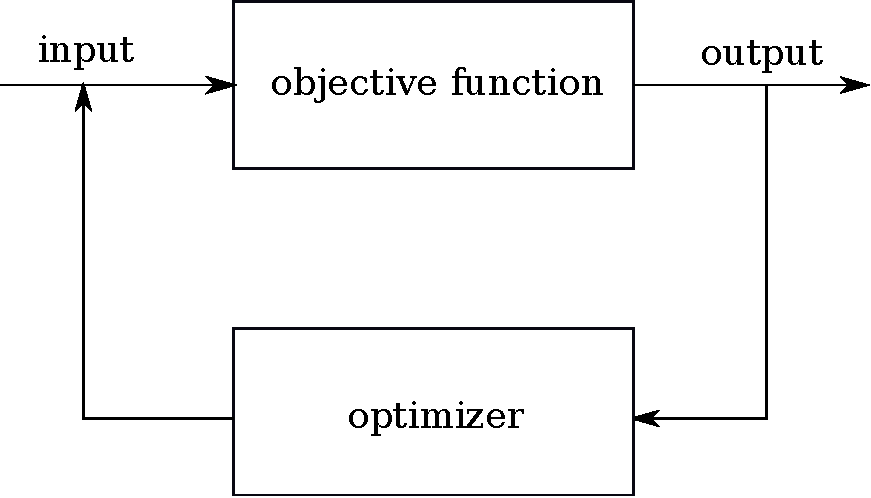
\includegraphics[width=3.2in]{black_box_optimization.pdf}
  \caption{This diagram shows the process of black box optimization. The task is to find a candidate solution (input) that can optimize (e.g. maximize or minimize) the objective function.}
  \label{fig:black_box_optimization}
\end{figure}

One of the promising application of evolutionary computation is black box optimization. Black box optimization refers to such problems that the optimization algorithm aims to optimize an objective function without assuming the hidden structure of that function (e.g., linear or differentiable). In particular, the aim is to found a set of inputs that can maximize or minimize the output of the objective function. For example, in a traveling salesman problem (a combinatorial optimization), in which the task is to find the best combination of route of cities (input) that can minimize the length of tour of visit all cities (objective). Fig.~\ref{fig:black_box_optimization} shows a diagram of the black box optimization.

Due to the complexity of the real problem in nature, the stochastic search algorithm such as evolutionary algorithms provide us an efficient and relatively `perfect' solutions. Although evolutionary algorithms could not guarantee the best solution would be found every time, they are still superior to many traditional search algorithms such as the greedy local search algorithm~\cite{Gutin200281}. There are many real-world examples that using evolutionary computation techniques to solve the optimization problem. In the area of nanophotonic light trapping, an urgent need is the development of low cost thin film solar photovoltaic technologies. A traditional way is fixing the structure according to the physical intuition and trying to find the optimal parameters. In~\cite{Wang2013}, a highly efficient light-trapping structure was designed using a genetic algorithm. It was shown that this new structure can increase the trapping efficiency three times comparing with the classic limit. The high efficiency achieved by the new design is far beyond the reach of traditional design. Another successful example is using evolutionary algorithms to design antennas for NASA's Space Technology spacecraft~\cite{Hornby2011}, and one of the antennas was used in the mission. The antennas is a critical device for the spacecraft to communicate with the ground, as faulty communication may cause a lot of data lost or the crash of the spacecraft. The antennas designed using evolutionary algorithms are significantly better than those designed by human experts. Another advantage of using evolutionary algorithms for designing is once the fitness function was changed, it can quickly come up with another design can fit the purpose. 

In the following, we list several cases (but not all) that evolutionary computation could be applied to solve the `tough' optimization problem. 

\begin{itemize}

\item \textit{High-dimension} As the dimension, $n$, of the objective function increases, the search space increases exponentially. This is called ``curve of dimension'' by Bellman~\cite{Bellman1957}. For example, if we have to optimize a function that has $30$ dimensions, and each dimension only has $20$ parameters to be selected. For a grid search in which all the possible solution is evaluated, it will take $20^{30}$ evaluations. Suppose that each evaluation takes $1\mu s$, it would more than the $3\cdot 10^{31}$ years. However, if using evolutionary computation, it probably takes hours to find the optimal solution. 

\item \textit{Multi-Model} Multi-model means a system (function) has more than one optimums (e.g., Rastrigin Function). The one/s with the best fitness value is/are considered as global optimum/s, and the other are considered as local optimums. 
These local optimums around the global optimum/s are very misleading for the gradient-based search algorithms (e.g., \textit{hill climbing} algorithm), as the solutions may easily get trapped at the local optimums. Evolutionary algorithms are shown to be very efficient to find the global optimum/s. %For example, in the optimization of a multi-layer forward neural network, there may be multiple representations that could produce the same output because of the symmetrical structure of the hidden neurons.

\item \textit{Non-separable and non-differential} A function, $g(x_1, x_2, \cdots, x_n)$ is non-separable, if it can not be expressed as: $g(x_1, x_2, \cdots, x_n) = g(x_1)g(x_2) \cdots g(x_n)$. For the separable function, it would be much easier to optimize, as we can treat each variable separately. However, for non-separable system, the variables are normally coupled. Also, the function may not be differential, which makes many mathematical optimization algorithms (e.g., quasi-Newton BFGS algorithm~\cite{Dennis1977} or conjugate gradient algorithm~\cite{Shewchuk1994}). The state-of-the-art of the evolutionary algorithm for black box optimization in contentious domain is Covariance Matrix Adaptation Evolution Strategy (CMAES)\cite{Hansen2003}.

\item \textit{Multi-objective} When encountering real-world problem, we usually need to deal with multiple objectives, which need to be optimized simultaneously. For example, when designing a car, the engineers need to consider the shape, performance of the engines, and more importantly cost. As some of the objectives (such as performance and cost) are conflicting, the designer needs to find a Pareto optimal solution, in which none of the value of the objective functions can not be increased without considering decreasing the value of other objectives. Evolutionary multi-objective optimization is an efficient technique for generating such Pareto optimal solutions for multi-objective optimization problems. For a review, see~\cite{Fonseca1995}. 

\end{itemize}

\subsubsection{Evolutionary Robotics}\label{sec:evolutionary_robotics}

Another application of evolutionary computation is evolutionary robotics, in which the controller and/or morphology of the robots are automatically generated. The user considers the robot as a whole and only needs to specify the criterion which is represented by a fitness function. The fitness function could be single-objective or multi-objective. The aim is to optimize (minimize or maximize) the fitness using evolutionary algorithms. The normal procedure of evolutionary robotics is as follows. First, an initial population of random controllers are generated. Each controller are represented by a chromosome. If the controller is a neural network, the chromosome is a vector of real numbers. Each controller was imported into the robot(s), and the robot's performance when performing various tasks is measured and evaluated using the pre-defined fitness function. After some genetic operators (e.g. crossover, mutation), the `fitter' robot controller has a higher chance of being selected and generating offspring in the next generation. This process iterates until a good solution is found. 

In contract to evolutionary robotics, another method of designing robot controller and/or morphology is behavior-based approach, where the designer divides the whole system into several simple parts intuitively. These separate parts are then integrated all in once through a coordination mechanism---competitive or cooperative coordination~\cite{Brooks1986}. In competitive coordination, only one part has an effect on the output of the robot, while in cooperative coordination, several parts contribute to the output of the robot with different weights. The behavior-based method was shown to be very robust in many tasks such as gait control in locomotion and object transport. The challenge of designing robot controller and/or morphology using behavior-based method is it requires a lot of experience from the designer. Moreover, when the system is highly coupled, separating the whole design into different parts may not be a good strategy. However, evolutionary robotics provides the designer an alternative way of controlling the robot as a whole, rather than focuses on the details of each separate component. The synthesized control system is a result of self-organized process. %A schematic diagram showing the design process of evolutionary method and behavior-based method is shown in Fig.~\ref{}.

There are many control structure that can be adapted in evolutionary robotics. One popular structure is artificial neural network due to its simple representation and strong power of control. The tree-based structure like LISP is also very robust, and it is widely used in evolutionary programming~\cite{Koza:1992}. The \textit{building blocks} method was proposed by Brooks~\cite{Brooks92artificiallife}. However, these blocks are described using high-level languages, which are are suitable for evolution in the low level. Comparing with other control structures, artificial neural network have many advantages~\cite{Floreano_1997, Floreano2008:NN}. According to the types of behavior (e.g., simple perception or non-linear dynamic), we can choose different neural networks (forward neural networks and recurrent neural networks, etc.). Recent development reveals that we can even evolve the topology and weights of the neural networks~\cite{Kenneth2002}. 

There are two main research aims in evolutionary robotics: 1) engineering---developing the control strategy for robots; 2) biology---to understand the biological systems using simulated evolution. In engineering, a range of work has been presented, ranging from simple behaviors, such as phototaxis behavior, self-charging behavior to complex behaviors such as navigation and locomotion of robot with multiple degrees of freedom. In biology, evolutionary robotics is used as a tool to understand the general principles of evolution. It provides much more efficient and faster way to validate or even create hypothesis based on evolution in simulation or real robots, compared with the slow evolutionary process in nature. AVIDA~\cite{Bryson2013} and AEvol~\cite{Batut2013} are two computer software systems that are used for studying the evolution of bacterial. In hypothesis validation, evolutionary robotics was used as a tool to investigate some key issues in biology. For example, whether altruistic plays an important role in cooperation~\cite{montanier:inria2011,Waibel2011}, the conditions of emergence of communication during the evolution~\cite{Floreano2007514}, and how morphology and control are coupled~\cite{Auerbach:PLoS:2014}, coevolution of predator and prey~\cite{Cliff_1995, Floreano_1998}. 
%In the simulation or experiments, some interesting behaviors which are similar to those in nature can be found and analyzed. For example, in~\cite{Floreano_1998}, the predator tries to catch the prey, while the prey tries to escape from the predator. Both species evolve more and more complicated behaviors in order to compete with each other.

Using evolutionary algorithms to generate a desirable behavior/result requires a relatively large population size and certain number of generations. Therefore, performing evolution on the real robot would take plenty of time. The initial experiments may also cause damage to the robot itself or the environment the robot is operating on. Therefore, a lot of experiments/evaluations are performed in simulation. As the simulator can not match the reality, the controller generated in simulation may not work well in reality, causing \textit{reality} gap. Some work are done to reduce the \textit{reality gap}. In~\cite{Koos:TEVC:2013, Koos:IJRR:2013}, the author uses the transferability approach to increase the quality of controller generated in simulation through reducing the gap between simulation and reality. In~\cite{Floreano1996}, the evolution is even performed directly on the real robot to evolve the controller to perform navigation task. However, the battery is still a problem as it takes two weeks to evaluate $100$ generations. The addressed this issue through connecting a wire between the robot and the power station. 

Recently, a distributed online onboard evolutionary method (artificial embodied evolution) has received much attention~\cite{Watson2012, eiben:inria-00531455, Eiben:EI:2012}. In artificial embodied evolution, the population is distributed among different robots, and the gene exchange is done through \textit{mating}. Each robot only exchange its genes with its nearby neighbors. There is not central control over the group of robots. This approach is particularly suitable for the situation where the environment that the robots are operating on is not predictable or changing after deploying the robots. The robots need to evolve to adapt to the changing environment, while satisfying certain basic requirements inserted by the designers. A more challenging research area could be evolving both the morphology and controller of the robots in a distributed manner---\textit{evolution of things}~\cite{Eiben:Nature:2015}. This forms an open-end evolution among different artifacts, which is a process how living creatures evolve in real world. The fast development of 3D printing technique makes this method appealing~\cite{Tumbleston20032015}. 

\subsubsection{System Identification}

System identification which is about building the model of a hidden system through conducting a set of experiments is widely used in both academic and industrial areas \cite{Ljung_1999}. The experiments are conducted by a series of inputs into the system and the outputs corresponding to the inputs are collected. The process of system identification is to find a model that fits the inputs and output. It is composed of observed data, model structure, a criterion to evaluate different models according to the observed data, validation of the obtained model based on different data set, and revision of model if necessary. 

There are two system identification approaches: the offline approach and online approach. In the offline approach, the observation data is collected first, and the aim of modeling is to generate a model that fits the observed data. This method is often used when the data is easy to collect or the parameters and operating environment of the system do not change too much in a short time. However, in some cases, the parameters of the system are always changing due to different operating environment. That means the obtained model based on the previous observation data can not be applied to the new situation any more. In this case, the model should be updated using the new observed experimental data and online system identification method. The two approaches of system identification are shown in Fig.~\ref{fig:modeling_approaches}. Note that for some systems, there are only outputs.
 
\begin{figure}[!t]
  \centering
  \subfloat[]{
  	  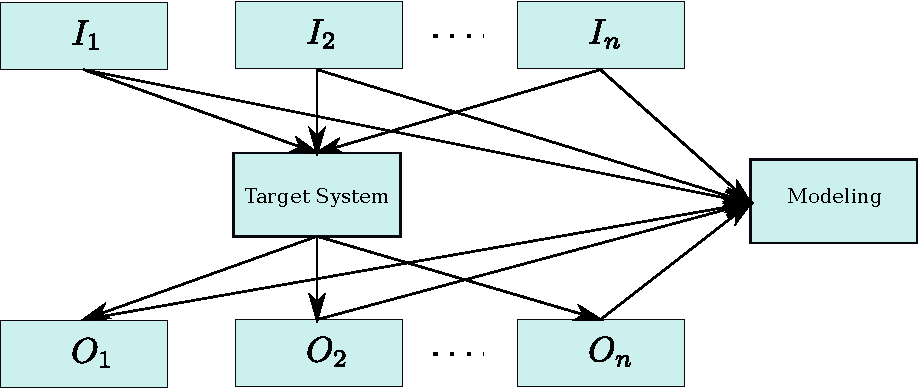
\includegraphics[width=2.5in]{system_identification_approach_offline.pdf}
  }\\
  \subfloat[]{
  	  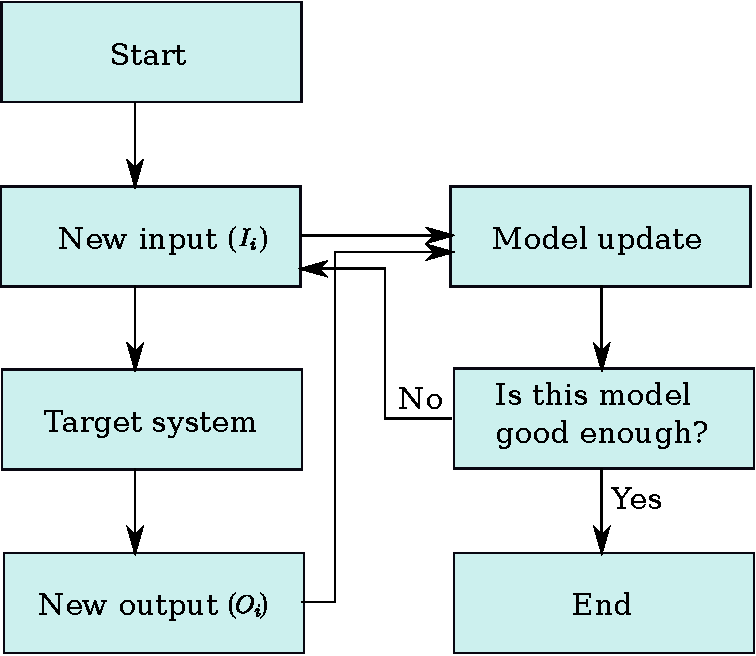
\includegraphics[width=2.5in]{system_identification_approach_online.pdf}
  }
  \caption{The diagram showing the two approaches ((a): offline; (b): online) for system identification. $(I_i, O_i)$, where $i \in [1, 2, \cdots, n]$, represents a pair of input data and output data.}
  \label{fig:modeling_approaches}
\end{figure}

System identification can be divided into two main procedures: modeling and estimation. Modeling defines the order or general structure of the hidden system \cite{Fogel_1991}. Estimation identifies the parameters associated with the given structure. There are many estimation algorithms to determine the parameters for a given structure. Typical estimation algorithms are recursive prediction error methods which are based on gradient search. Gradient search method such as greedy algorithm can easily get trapped in local optima, especially when there are numerous local optimal points near the global optima. An alternative search method is using evolutionary algorithms. As evolutionary algorithms use population-based search method, this makes it more likely to get rid of local optima. 

There are also some system identification methods that combine the modeling and estimation process, e.g., NARMAX method~\cite{Billings2013}. Neural network is a good representation of the system under investigation, as its topology and weights can be optimized simultaneously. The disadvantage of neural network is it is hard to interpret the obtained model when there are multiple layers, which makes it much hard to analyze the target system. Genetic programming provides an alternative way for finding the structure and parameters of the system. The model represented by genetic programming is described in a tree-based structure. As the structure in genetic programming is evolving, the obtained model may have different structure in different runs~\cite{Vladislavleva:2009}. Bloating is a problem in genetic programming, where the growth of the tree increases the complexity of the model structure. 

Coevolutionary algorithms provide an effective way for system identification~\cite{Bongard2005}, \cite{Bongard_remote_robot_2004,Bongard_function_recovery_2004,Koos2009,Bongard2007PNAS,Mirm2011,Ly2014}. A range of work have been performed on simulated agents. In~\cite{Bongard_remote_robot_2004}, Bongard and Lipson proposed the \emph{estimation-exploration algorithm}, a nonlinear system identification method to coevolve inputs and models in a way that minimizes the number of inputs to be tested on the system. In each generation, the input that leads to the highest disagreement between the models' predicted output in simulation was carried out on the real system. The quality of the models was evaluated through quantitatively comparing the output of the real system and the models' prediction. The method was applied to evolve morphological parameters of a simulated quadrupedal robot after it undergoes `physical' damage. In a later work~\cite{Bongard_function_recovery_2004}, they reported that ``in many cases the simulated robot would exhibit wildly different behaviors even when it very closely approximated the damaged `physical' robot. This result is not surprising due to the fact that the robot is a highly coupled, non-linear system: thus similar initial conditions [...] are expected to rapidly diverge in behavior over time''. They addressed this problem by using a more refined comparison metric reported in~\cite{Bongard_function_recovery_2004}. In~\cite{Koos2009}, an algorithm which is also based on coevolution of models and inputs was presented to model the simulated quadrotor helicopter and improve the control quality. The inputs were selected based on multiobjective performances (e.g., disagreement ability of models as in ~\cite{Bongard_remote_robot_2004} and control quality of a given task). Models were then refined through comparing their prediction to each selected test trajectory. In~\cite{Kouchmeshky_2007}, the damage detection process is conducted by coevolutionary algorithm to extract the maximum information from the system. In \cite{Mirmomeni_2011}, coevolutionary algorithm is applied to estimate chaotic time series, in which the test data that can extract information from the chaotic system co-evolves with the models. In these works, predefined metrics are critical for evaluating the performance of models. 
  
Many studies also investigated the implementation of evolution directly in physical environments, on either a single robot~\cite{ Bongard-etal2006:science, Koos2013, Cully2015} or multiple robots~\cite{Alan2014}. In~\cite{Bongard-etal2006:science}, a four-legged robot was built to study how it can infer its own morphology through a process of continuous self-modeling. The robot ran a coevolutionary algorithm on-board. One population evolved models for the robot's morphology, while the other evolved actions (inputs) to be conducted on the robot for gauging the quality of these models through comparing sensor data collected. In~\cite{Alan2014}, a distributed coevolutionary approach was presented to coevolve on-board simulators and controllers of a swarm of ten robots to perform foraging behavior. Each robot has its own simulator which models the environment. The evolution of each robot's simulator was driven by comparing the real-world foraging efficiency (a pre-defined fitness metric) of its nearby neighbors each executing the best controller generated by their own simulators. Each robot has a population of controllers, which evolved according to the robot's on-board simulator. The best controller was chosen for performing real-world foraging. This physical/embodied evolution helps reduce the \textit{reality gap} between the simulated and physical environments~\cite{Jakobi95}. In all of the above approaches, the model optimization is based on pre-defined metrics (explicit or implicit), which are task dependent.

%In \cite{Kouchmeshky_2007}, the damage detection process is conducted by coevolutionary algorithm to extract the maximum information from the system. In \cite{Mirmomeni_2011}, coevolutionary algorithm is applied to estimate chaotic time series, in which the test data that can extract information from the chaotic system co-evolves with the models. The approach described in~\cite{SchmidtLipson2009:science}, where the authors infer physical laws from observing mechanical systems, would also be applicable to learn about the behavior of an animal. Different from this approach our system learns about the behavior not through passive observation, but rather through an interactive process.

\section{Combining AI/Robotics and Animal Behavior}\label{sec:combine_AI_robotics_animal_behavior}

The variety of animal behaviors in nature is immense, ranging from simple perception to complicated behaviors such as navigation and communication. The scientific study of animal behavior is pursued not only because it is a subject of interest in itself, but also because the knowledge gained from it has several practical applications. In AI/Robotics, there is a large interest of studying animal behavior, as the model/knowledge learned can be used to build a more intelligent machine. At the same time, building machine that mimics the animal helps us better understand its behavior. In this section, we review how AI/robotics and animal behavior study benefit each other. In Section~\ref{sec:animal_behavior_in_nature}, we introduce some interesting animal behaviors observed in nature. In Section~\ref{sec:swarm_optimization_swarm_robotics}, we detail how the animal behavior observed in nature can be used as inspiration for solving engineering tasks, especially in the area of AI/robotics. In Section~\ref{sec:contribution_of_AI/robotics_to_ethology}, we show how AI/Robotics can contribute to the study of animal behavior, which is the theme of this thesis.

\subsection{Animal Behavior in Nature}\label{sec:animal_behavior_in_nature}

\subsubsection{Single Behaviors}

Comparing with the behaviors exhibited by complex animals such as mammals, insect behavior arises a large interest both by biologists and roboticists. One reason is due to the simple neural system of the insects, which provides a good inspiration for engineering purpose. This simplicity also makes it easy to replicate the intelligence exhibited by the insects. 

A basic insect behavior is taxis, which is its intrinsic behavioral response to a specific stimulus. Taxis is divided into different type according to the stimulus which elicits the response. These behaviors include phototaxis (light), chemotaxis (chemicals), thermotaxis (temperature), etc. For example, a lobster follows the salt-water plume---a kind of chemical signal to find its source. Another interesting taxis behavior of crickets is that the female crickets perform complex auditory orientation behavior towards the male crickets. Researchers have found this complex sound localization behavior emerge from simple reactive steering responses to specific sound pulses generated by male crickets~\cite{Hedwig2004}. Apart from taxis behaviors, some insects use the stimuli as cues for navigation or migration. For instance, the bee uses its vision system to navigate in the air and avoid obstacles. Another interesting behavior found in insects is the ball movement of dung beetles~\cite{Emily_2012}. Once the dung beetles form the pieces of dung into a ball, they always roll the dung-ball in a straight line using various stimuli (e.g., the moon, sun and polarised light \cite{Byrne_2003, Matthews_1962}) as visual cues to transport the food source. This behavior ensures that they keep away from the competitors as far as possible. 
 
The stimulus-response behaviors in insects mentioned above are investigated by biologists for centuries. When investigating such behaviors, biologists need to learn how to interact with the animal in a meaningful way to extract all the behavioral repterio of the insect under investigation. However, whether this interacting ability could be exhibited by an intelligent machine is still an uncertain problem, which is addressed in this thesis. 

\subsubsection{Swarm Behaviors}

Apart from single-animal behavior, swarm behaviors, which are emergent (collective) behaviors that arise from the interactions of a number of animals (especially social insects) in a group, have also been widely observed in nature. The individual behaviors in a swarm tend to be relatively simple~\cite{Camazine2001}. The global behavior that is exhibited in a swarm is a result of self-organized process. Researchers found that individuals do not need the representation or complex knowledge to build a map of what the global behavior should be~\cite{Garnier:SI:2007}. There are no leaders in the colony. From the point of control, swarm behavior is a distributed control system which does not rely on central coordination.

Many swarm behaviors are observed in nature. For example, the flocking behavior of birds are of particular interest to humans. This is not only because of their beautiful shape formed in a group, but also how the birds coordinate with each other to maintain that shape. A simple mathematical model was proposed by~\cite{Craig:CG:1987} to describe the individual behavior of each bird in a flocking. The three rules are: attraction, repulsion and alignment. In the attraction rule, the birds will be attracted by their neighbors, and this would result in each bird moving towards to the `center' of their neighbors. Repulsion means the bird needs to avoid colliding with each other. Alignment assumes that each bird moves in the same direction with its neighbors. Although there is no prove that flocking birds follow exactly these three rules, it is attractive that the boids (in simulation) following such simple rules can mimic the real flocking behavior very closely. There are many some other swarm behaviors which are also studied extensively such as the aggregation of cockroaches~\cite{Jeanson:AB:2005}, foraging in ants~\cite{Carroll1973}, flashing synchronization in fireflies~\cite{James:ARE:1971}, mound building in termites~\cite{Bruinsma:PHD:1979}. 

\subsection{Swarm Optimization and Swarm Robotics}\label{sec:swarm_optimization_swarm_robotics}

In the previous sections, we introduce some interesting animal behaviors observed in nature. Many algorithms are inspired from observation of animal behaviors. In this section, we will review two main optimization algorithms inspired from swarm behaviors---ant colony optimization algorithm~\cite{Dorigo_1997} and particle swarm optimization algorithm~\cite{Kennedy:ICNN:1995}. Swarm robotics is another application area which uses the swarm behaviors of social animals as an inspiration to solve complex tasks using multiple robots. 

\subsubsection{Swarm Optimization}

\textbf{Ant Colony Optimization}

Ant Colony Optimization (ACO) is an optimization technique that gets inspiration from foraging behavior of ants. When ants go out to search for food, they will leave pheromone in the path. Ants will be attracted by the pheromone, the strength of which represents the quality of the food source. Researchers have found that this indirection communication, which is know as \textit{stigmergy}~\cite{Holland:AL:1999}, leads them to found the shortest path along their nest and location of food source. The initial application of ACO is to find the optimal path in the combinational (discrete) problem. Note that nowadays the application of ACO algorithms ranges from network optimization (e.g., routing and load balance~\cite{DiCaro:JAIR:1998}) to continuous optimization~\cite{Dorigo:LNCS:2004}.   

The principle of ACO algorithms can be divided into the following two steps:

\begin{itemize}
\item Use the pheromone model to generate condidate solutions. From the aspect of mathematics, the pheromone model is a parameterized probability distribution in the search space.

\item The candidate solutions are used as a bias for the future sampling to get better solutions.
\end{itemize}

\textbf{Particle Swarm Optimization}

Particle Swarm Optimization (PSO) is another an optimization algorithm which gets inspiration from flocking of birds or schooling of fish. It was first proposed by Kennedy and Eberhart~\cite{Kennedy:ICNN:1995}. The initial application is to optimize the weights of neural networks---a continuous optimization problem. It is also widely used in discrete optimization. 

The basic component in PSO is called \textit{particle}. A PSO algorithm consists of a finite set of particles. The movement of each particle is updated using \textit{velocity}. The velocity of each particle in each time step is updated based on its current velocity, the deviation between the best position (it has found so far) and its current position, and deviation between the best position by its neighbors and its current position. This will result in the particles moving towards the high-quality solutions after certain iterations. The update of each particle can be written using two equations as follows:
\begin{equation}\label{eq:particle_velocity_update}
\overrightarrow{v}_{i+1} =  \overrightarrow{v_{i}} + c_1\overrightarrow{R_{1}}\otimes(\overrightarrow{p_{i}} - \overrightarrow{x_{i}}) + c_2\overrightarrow{R_{2}}\otimes(\overrightarrow{p_{g}} - \overrightarrow{x_{i}}) 
\end{equation} 

\begin{equation}\label{eq:particle_position_update}
\overrightarrow{x}_{i+1} =  \overrightarrow{x_{i}} + \overrightarrow{v_{i}}
\end{equation} 

where $\overrightarrow{R_{1}}$ and $\overrightarrow{R_{2}}$ are independent random number generators that return a vector of random values in range $[0, 1]$. $c_1$ and $c_2$ are referred to as acceleration coefficients. The first item in Eq.~\eqref{eq:particle_velocity_update} keeps the particle moving in the previous direction; the second item makes the particle move towards the best position of its own; the third position forces the particle move towards to the best position that its neighbors have found. Eq.~\eqref{eq:particle_position_update} updates the particle's position.  

\subsubsection{Swarm Robotics}

In the previous sections, we talk about how swarm behaviors can be used as inspiration for algorithms design. In this section, we introduce how to use swarm intelligence techniques to multiple robots research, which is referred to as swarm robotics. Many social insects' (e.g, ants, termites, wraps and bees) behavior can be used as inspirations in swarm robotics. 

Swarm robotics investigates how multiple robots each with limited ability communicate, coordinate and self-organize to accomplish complex tasks. To finish the same task, using a single expensive robot with complex control structure may be feasible but it may have low efficiency and prone to failure. The advantages of swarm robotics are as follows: 

\begin{itemize}

\item \textit{Robustness} A swarm system consisting of multiple robots is robust in term of failure of certain robots disturbance of the environment. This robustness can be explained in the following reasons: 1) if some robots failed, the other robots would replace the functions of the failed robots; 2) the control is distributed; 3) as the individual is simple, it is less likely to be damaged; 4) the perception from multiple robots would increase the system's robustness. Note that in some swarm systems, there may be exceptions. That is, some individual failure would influence the whole self-organized process~\cite{Bjerknes2013}.

\item \textit{Scalability} In swarm robotics, the number of robots do not have significant difference on the global performance/behavior in the system. That is, increasing/decreasing certain number of robots, the system is still under control and the coordination is maintained. When investigating a swarm robotic system, scalability study is usually considered~\cite{Jianing:TRO:2015, Melvin_DARS2014}.

\item \textit{Flexibility} The swarm could easily adapt to the changing tasks and generate relevant solutions~\cite{Sahin:LNCS:2005}. The role of each robot in the swarm could be changed depending the need for the task. 
\end{itemize}

In order to cooperate, the robots need to interact with each other and environment. There are three kinds of interaction in swarm robotic systems. 

\begin{itemize}

\item \textit{interaction via environment} In this interaction method, the robots communicate with each through changing the environment. There is no explicit communication between each robot (i.e., they do not exchange message). In nature, this method is observed in social ants. The pheromone they leave when foraging is an environmental stimulus for locating the food source.  

\item \textit{interaction via perception} In this method, the robots can perceive each other in a limited range. This perception is local and there is no explicit communication between each robot. This requires the robots can distinguish between robots and objects in the environment. In nature, when the ants need to collectively pull the food to the nest, they need to perceive each other (to avoid collision) and the food (object).

\item \textit{interaction via explicit communication} In this method, a network is required to communicate with a swarm of robots in real time. This could be done by broadcast (e.g., WiFi~\cite{Gerkey:TRA:2002}) or a distributed sensing network~\cite{Winfield:LNCS:2000}. How to build a reliable network when the number of robots is significantly large is still a hot topic widely discussed. When the number of robots increases, the load of communication increases exponentially. A possible solution is combining the advantage of network communication and local communication using the robots' perception.

\end{itemize}

A range of tasks have been demonstrated in swarm robotics. The tasks range from aggregation~\cite{Trianni:LNCS:2003, Gauci2014_ijrr, Garnier:AL:2008, Jeanson:AB:2005}, dispersion~\cite{howard2002mobile, mclurkin2004distributed}, pattern formation~\cite{Fujibayashi:DARS:2002, Chen:AAMAS:2012}, collective movement~\cite{Turgut:SI:2008} to cooperative transport~\cite{Kube:AB:1993, Kube:RAS:2000,Gross:IJBC:2009, Jianing:TRO:2015}, etc. Aggregation can be considered as the fundamental behavior of other more complex tasks. In~\cite{Jeanson:AB:2005}, a group of robots mimic the cockroaches' aggregation behaviors, in which the robots gather into or leave the nest with a probability proportional to the size of the nest. The advantage of using stochastic algorithm is that they do not need to form a connected network in the initial configuration. In~\cite{Gauci2014_ijrr}, the robots each with a binary sensor were reported to aggregate into a single cluster, validated using $40$ e-puck robots. The robots do not need to perform algorithmic computation. This work was scaled well using $1000$ robots in simulation. In~\cite{Werfel:Sci:2014}, Werfel et al. designed a group of termite-inspired robots that work collectively to build several structures. The robots communicate with each other using \textit{stigmergy}. In~\cite{Turgut:SI:2008}, a group of nine Kobot robots were reported to mimic the flocking behavior of birds. These robots followed some simple rules similar to those proposed by Reynolds~\cite{Craig:CG:1987}. In cooperative transport, Chen et al.~\cite{Jianing:TRO:2015} proposed a strategy in which the robots only push the object when the robots' vision of the goal is occluded by the object. This strategy was proved to push any convex object in a plenary environment. 

\subsection{Contribution of AI/Robotics to Ethology}\label{sec:contribution_of_AI/robotics_to_ethology}

In the previous sections, we reviewed how animal behavior study can be used as inspiration for designing algorithms and robotic systems. However, robotics can also benefit animal behavior study. In this section, we review two approaches in AI/robotics to contribute to the study of animal behavior: \textit{learning from synthesis} and \textit{robot-animal interaction}.

\subsubsection{Learning from Synthesis}

Ethologists have studied animal behavior over a century. However, even some basic behaviors such as taxis (which is widely observed in animals such as insect larvae and worms~\citep{Fraenkel:DP:1961, Stephen:Op:1990}) is still not completely understood \cite{Rano_2009}. There are some basic steps that ethologists follow in the study of animal behavior~\cite{camazine2003self}. The first step is observation, and after that they formulate some scientific questions on the observed behavior, and generate hypothesis to answer these questions. In order to verify the hypothesis, they actively conduct related experiments in the real animals and collect certain amount of data. After analyzing the data, the conclusion will be made to support or reject their hypothesis.

Robotics or artificial life can be used as an alternative methodology to investigate and understand animal behavior. Robots can be used as physical models of animal behaviors for testing hypotheses~\citep{Barbara_2000, Meyer2008}. For example, taxis behavior has often been implemented on mobile robotic systems. Webb~\citep{Barbara_1995} used a robot to model the phonotaxis behavior of crickets~\citep{Popov:JCP:1997}. The robot can locate the position of a sound source and move towards it under different conditions. There was a good agreement between data collected from experiments on the robot and the animal. Another taxis behavior---chemotaxis in which animals follow a specific chemical trial has been used as a model for robots to find odour source based on artificial neural networks \cite{Farah_2002} and even Braitenberg vehicles \cite{Lilienthal_2003}. Robots can be used as a validation for the models obtained from biologists and allow them to better understand the animal behavior from a synthetic point of view.  Besides, roboticists can generate new hypotheses and test them using (simulated or real) robots.
 
In social behaviors study, Balch et al.~\citep{Balch_2006} built executable models of the behaviors and ants and monkeys, which can be directly executed by multi-robot systems. The aim is to show how research into multi-robot systems can contribute to the study of collective animal behaviors. Besides robotics, there are some researchers arguing that artificial intelligence can also make significant contributions to biological study. In \cite{Chappell_2010}, Chappell et al. argue that there are many ways in which biologists interested in natural intelligence can learn from AI, and they outline the many specific kinds of contributions that AI can make to biological study. They also give some suggestions on how AI researchers collaborate with biologists to combine the advantage of each other and solve some cutting-edge problems in animal behavior.

As opposed to the works mentioned above, the method proposed in this thesis aims to synthesize models of animal (agent) behaviors automatically, rather than manually. This could help to spare scientists from having to perform numerous laborious experiments, allowing them instead to focus on using the generated models to produce new hypotheses and conduct further experiments. 

\subsubsection{Robot--Animal Interaction}\label{sec:robot_animal_interaction}

Besides pure robot-based or AI research, researchers also use robots to interact with real animals. They build and programme robots (i.e., replicas) that can be inserted into the group of social animals~\cite{Faria2010, Halloy2013, J.Halloy2007, Thomas2013, Vaughan2000}. Robots can be created and systematically controlled in such a way that they are accepted as con- or hetero-specifics by the animals in the group~\cite{Krause2011}. In this case, one ``animal'' in a group is completely controlled and they can observe the behaviors of the mixed society \cite{J.Halloy_2007}. The behavior of the inserted robot can be controlled and the model can also be embedded into the robot for verification \cite{Krause_2011}. The behavior of robots can be programmed in such a way that its behavior is not influenced by the other real animals in the group, and they can be used as demonstrators or leaders in the experiments. Further more, it is easier to verify a hypothesis through controlled interaction in social behaviors. 

For example,  in~\cite{Faria2010}, a replica fish which resembled the appearance (i.e., visual morphology) of sticklebacks was created to investigate two types of interaction: recruitment and leadership. In~\cite{J.Halloy2007}, autonomous robots which executed the derived model were mixed into a group of cockroaches to modulate their decision-making of selecting shelter in the aggregation behavior. The robots behaved in a similar way to the cockroaches. Although the robots' appearance was different to that of the cockroaches, the robots released a specific odor that the cockroaches could detect and regard the robots as conspecifics. In \cite{Vaughan_1998, Vaughan2000}, Vaughan et al. have built a mobile robot that can interact with the ducks in a circular arena and drive them to the safe place. Halloy et al. In \cite{Gribovskiy_2010}, Gribovskiy et al. designed a robot which is capable of interacting with chicks to study how the behavior of chicks can be influenced by the others in a group. Although robots which are well designed can be mixed in social animals, building such kind of robot is a time-consuming process. It is also expensive to some extent and requires the collaboration of researchers from different disciplines. In~\citep{Kopman2013}, a robot-fish that can interact intelligently with live zebrafish to study their preference and locomotion behavior was designed . 

In these works, the models were manually derived and the robots were only used for model validation. We believe that this robot-animal interaction framework could be enhanced through \textit{Turing learning}, which autonomously infers the collective behavior. 

\clearpage 

%The research of animal behavior has lasted for centuries. There are some basic steps that ethologists follow in the study of animal behavior. The first step is observation, and after that they formulate some scientific questions on the observed behavior, and generate hypothesis to answer these questions. In order to verify the hypothesis, they actively conduct related experiments in the real animals and collect certain amount of data. After analyzing the data, the conclusion will be made to support or reject their hypothesis. Take the behavior of dung beetle for instance. An interesting feature observed by ethologists in the behavior of dung beetles is that they always roll the dung-ball in a straight line. This strategy guarantees that the beetles can roll the dung as far as possible in the shortest time, ensuring that they can escape from the competition or danger that may occur near the cite of dung \cite{Emily_2012}. Previous works show that the most significant cues which dung beetles use for navigation -- straight line movement are the moon, sun and polarised light \cite{Byrne_2003, Matthews_1962}. In \cite{Dacke_2004}, Dacke, et al. study how dung beetle \textit{Scarabaeus zambesianus} orientates due to the artificial polarization pattern instead of observing the behavior in the natural polarized light, since it is quite easy to control the angle when using artificial light source. To do the experiment, they put the dung beetle in a squared arena. When the beetle enters the central point, they switch the angle of the artificial light source from 0 degree to 90 degree to interact with the dung beetle. Then they observe the path taken by the rolling dung to see whether the angle of light source has influence on the beetle's orientation behavior. The light switching process is very time-consuming, and the researchers have to change the angle of light source for many times (90 times, if the angle increases one degree each time). However, if this process is finished by a machine, it could free the ethologists from a lot of repetitive tasks, since the machine can shift the angle of light source as a grid of numeric values and observe the orientation of dung beetle under each specific condition. A high-capacity machine could observe this behavior without human intervention, generating thousands of experimental data very quickly. 